\chapter{Diseño del agente}

En este capítulo se detallará el diseño del agente propuesto para la resolución del problema. 

Se empezará presentando la formalización del conocimiento usada (estado, acción y recompensa) y las características físicas del agente. Tras esto, se describirán las dos arquitecturas propuestas para el agente: una primera basada en una red neuronal convolucional, y una segunda basada en una red profunda híbrida. Finalmente, se explicará el proceso de actuación y entrenamiento del agente.

\section{Caracterización del conocimiento}

En esta sección se describe la caracterización del conocimiento realizada, centrándose en los puntos principales del aprendizaje por refuerzo: el \textbf{estado}, las \textbf{acciones} disponibles y las \textbf{recompensas} que recibe el agente. Además, se describen las características del agente propuesto dentro del entorno \textit{Habitat}.

\subsection{Características del agente físico en \textit{Habitat}}

Las características del agente físico simulado son las siguientes:
\begin{itemize}
	\item \textbf{Forma física del agente:} La forma del agente es un \textbf{cilindro} de $1.5$ metros de altura y $0.1$ metros de radio.
	
	Esta forma física no se corresponde a ningún robot real, siendo la del agente por defecto simulado por \textit{Habitat}.
	\item \textbf{Capacidad de movimiento:} El agente únicamente es capaz de desplazarse hacia delante, pudiendo moverse $0.25$ metros en cada paso simulado.
	
	Para cambiar la dirección de su movimiento, el agente necesita rotar sobre si mismo. Ésto lo hace en intervalos de $10$ grados en cada paso simulado. El agente no puede girar y desplazarse en el mismo paso.
	\item \textbf{Sensores disponibles:} El agente cuenta con acceso a los siguientes sensores:
	\begin{itemize}
		\item \textbf{Cámara de profundidad:} Una cámara de profundidad (\textit{DEPTH{\_}SENSOR)} situada a una altura de $1.25$ metros respecto al suelo, apuntando a la dirección en la que se desplaza el agente.
		
		Esta cámara genera imágenes de profundidad de $(256x256)$ píxeles con valores en el rango $[0.0, 1.0]$. La cámara tiene un ángulo de visión de $90$ grados, y es capaz de detectar objetos hasta una distancia de $10$ metros.
		\item \textbf{Brújula y GPS (\textit{POINTGOAL{\_}WITH{\_}GPS{\_}COMPASS{\_}SENSOR}):} Una brújula y un GPS que conocen la posición exacta de la meta en todo momento. Estos sensores ofrecen el \textbf{ángulo} y la \textbf{distancia euclidiana} hasta la meta en forma de valor decimal.
	\end{itemize}
	\item \textbf{Métricas usadas:} El agente ofrece las siguientes métricas para su evaluación posterior:
	\begin{itemize}
		\item \textbf{Distancia hasta la meta}: Un valor numérico que indica la distancia euclidiana hasta la meta (la distancia euclidiana entre el agente y la meta) en metros.
		\item \textbf{Éxito:} Un valor booleano que indica si el agente está en la meta (verdadero) o falso. El agente se considera en la meta si se encuentra a menos de $0.3$ metros de esta.
		\item \textbf{\textit{SPL} y \textit{Soft SPL}:} Dos valores numéricos que indican la métrica de \textit{Success weighted by Path Length} \cite{DBLP:journals/corr/abs-1807-06757} y su variante suavizada. Ambas fórmulas fueron definidas en el Capítulo 4.
	\end{itemize}
\end{itemize}

\subsection{Estado}

El \textbf{estado} (la percepción que tiene el agente del entorno) consta de tres elementos:

\begin{itemize}
	\item \textbf{Imagen de profundidad:} Una imagen en escala de grises representando las observaciones de la cámara de profundidad. Esta imagen tiene un tamaño de $(256 x 256)$ píxeles, con los valores de cada celda en el rango $[0.0, 1.0]$ (donde $0.0$ o negro significa cercanía a la cámara y $1.0$ o blanco significa lejanía). Se puede ver un ejemplo de la imagen en la Figura \ref{fig:chap5-estado}.
	
\begin{figure}[h]
    \centering
    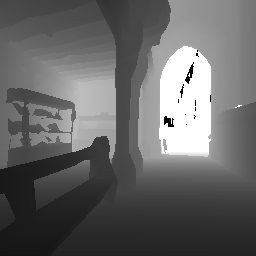
\includegraphics{imagenes/cap5/normalized.png}
    \caption{Ejemplo de imagen de profundidad usada como parte del estado.}
    \label{fig:chap5-estado}
\end{figure}			
			
	Se ha optado por añadir este valor debido al planteamiento del problema. Al buscar diseñar un agente reactivo frente a obstáculos, es importante que el agente sea capaz de percibir cualquier objeto que se encuentre en su camino. Una cámara de profundidad nos permite estimar las distancias a estos obstáculos de forma rápida y simple.	
	

	\item \textbf{Distancia a la meta:} Un valor decimal que representa la distancia actual entre el agente y la meta en metros.
	
	Este valor forma parte del estado al ser parte del cálculo de la recompensa (como se verá posteriormente). Además, es importante que el agente sea capaz de estimar la distancia hasta la meta para que tenga la posibilidad de aprender cuando detenerse.
	
	\item \textbf{Ángulo respecto a la meta:} Un valor decimal que representa el ángulo que debería girar el agente para enfocarse hacia la meta, en radianes. Un valor positivo significa que el agente debería girar hacia la derecha, mientras que un valor negativo significa que el agente debería girar hacia la izquierda.
	
	Si bien este valor no forma parte del cómputo de la recompensa, se ha optado por añadir el ángulo al estado para permitir al agente tener la posibilidad de aprender información respecto a su orientación que no podría aprender en otro caso.
\end{itemize}

Si bien se consideró añadir una \textbf{imagen en color} al estado, finalmente se ha optado por no incluirla. Esto se debe a que la información que añade resulta superflua, ya que la cámara de profundidad incluye toda la información necesaria para el cálculo de obstáculos. Además, los escenarios de interior son complejos con altos niveles de ruido, por lo que una cámara de color podría llevar a sobreajustes (al aprender el aspecto de los interiores frente a los obstáculos).

Un estado se considera \textbf{final} cuando el agente lo finaliza (ya sea por realizar la acción específica de terminar o por superar el número máximo de acciones permitidas). Este estado final puede ser \textbf{exitoso} si la distancia a la meta es menor a un umbral (por defecto $0.3$ metros), o \textbf{fallido} en otro caso.

\subsection{Acciones}

El agente es capaz de realizar \textbf{cuatro} acciones en total:

\begin{itemize}
	\item \textbf{Desplazarse} hacia delante. Por defecto, el desplazamiento es de $0.25$ metros.
	\item \textbf{Girar} hacia la derecha o la izquierda. Por defecto, el giro es de $10$ grados.
	\item \textbf{Finalizar el episodio}. La inclusión de una acción para finalizar el episodio es una de las principales sugerencias de Peter Anderson \textit{et al.} \cite{DBLP:journals/corr/abs-1807-06757} para la evaluación de agentes físicos.
\end{itemize}

Como se comentó en el Capítulo 2 y se puede observar, el agente no es capaz de un movimiento omnidireccional (como sí podría un dron volador). El agente únicamente puede desplazarse hacia adelante, necesitando rotar sobre sí mismo para cambiar la dirección de su movimiento.

\subsection{Recompensas}

El sistema de recompensas diseñado está basado en el sistema originalmente propuesto por Carlos Sampedro \textit{et al.} \cite{Sampedro2018}, siendo éste un sistema de recompensas basado en campos de potenciales artificiales, con un \textbf{atractor} que atrae al agente hacia la meta y \textbf{repulsores} que repelen al agente de los obstáculos. Ahora bien, este sistema ha sido adaptado a la arquitectura del agente desarrollado (con cámara de profundidad), y se han propuesto variantes para evaluar su rendimiento.

El cálculo de la recompensa de un estado se puede dividir en los siguientes pasos:
\begin{enumerate}
	\item Preprocesamiento de la imagen del estado.
	\item Identificación de obstáculos en la imagen (con dos posibles métodos)
	\item Cálculo de los potenciales atractivos y repulsivos.
	\item Cálculo de la recompensa final (con dos posibles métodos)
\end{enumerate}

Estos pasos se describirán a continuación.

\subsubsection{Preprocesamiento de la imagen de profundidad}

Para calcular las recompensas posteriormente, es necesario identificar los obstáculos o los objetos que pueden suponer un riesgo en la imagen. Ahora bien, no se puede usar la imagen directamente al contener ruido e información necesaria. Por esto, se realiza un preprocesamiento antes de identificar los obstáculos en la imagen, siguiendo los siguientes pasos:

\begin{enumerate}
	\item \textbf{Normalización:} Por defecto, la imagen obtenida por la cámara está formada por valores decimales en el rango $[0.0, 1.0]$. Ahora bien, para poder trabajar por la imagen es necesario que estos valores sean enteros en el rango $[0, 255]$ por compatibilidad con otras librerías. Por tanto, se transforman los valores de un rango al otro.
	\item \textbf{Recorte de los extremos:} Se ha visto que los extremos superiores e inferiores de la imagen (el suelo y el techo) no aportan información útil a la hora de calcular la recompensa, pudiendo llegar a introducir ruido y obstáculos que no existen.
	
	Para evitar esto, se recortan los extremos superiores e inferiores de la imagen. Por defecto, se recortan $35$ pixeles de cada extremo. Este valor se ha obtenido de forma empírica con pruebas y es heurístico.
	\item \textbf{Eliminación de artefactos del simulador:} En ocasiones, el simulador introduce ruido en la imagen en forma de partes de color negro puro (con valor $0$). Estos artefactos no son reales (al no ser capaz la cámara de devolver un valor tan bajo en la práctica) y pueden interferir con la detección de obstáculos, por lo que es necesario eliminarlos.
	
	Para eliminarlos, se sustituyen todos los valores de $0$ (negro puro) por $255$ (blanco puro). Esto hará que sean ignorados en los pasos posteriores.
	
	\item \textbf{Umbralización (\textit{Thresholding}):} Es necesario identificar los obstáculos en la imagen. Si bien se podría haber optado por alguna técnica de búsqueda de contornos (como \textit{Canny}), se ha elegido realizar una umbralización, donde todos los valores de la imagen son reemplazados usando la siguiente fórmula:
	\[
		imagen(x) = 
		\begin{cases}
			1,& \text{si } imagen(x) \leq suelo(255*umbral)\\
			0,& \text{en cualquier otro caso} 
		\end{cases}
	\] 
	Donde $umbral$ es el valor que se ha tomado para umbralización en el rango $[0.0, 1.0]$ (siendo por defecto $0.15$, elegido de forma empírica).
	
	En esencia, esta fórmula sustituye todos los valores menores a $suelo(255*umbral)$ (cercanos a la cámara) por $1$ (blanco), mientras que el resto de valores (lejanos) son sustituidos por $0$. De esta forma, se obtiene una imagen binaria en la que solo se conservan los obstáculos más cercanos.
	
	\item \textbf{Eliminación de ruido:} El proceso de umbralización puede crear ruido, como pueden ser regiones negras pequeñas dentro de contornos blancos más grandes, que pueden afectar al rendimiento.
	
	Para eliminar este ruido, se usa una técnica de \textit{apertura morfológica}, que consiste en una dilatación (aumentar el volumen de los objetos en la imagen) seguida de una erosión (disminuir el volumen de los objetos en la imagen). Esto reduce el ruido incluido dentro de los contornos, sin afectar demasiado al volumen final.
	
	\item \textbf{Dilatación:} El paso final consiste en dilatar (aumentar el volumen) de la imagen, para evitar perdidas de información provocadas por la eliminación de ruido del paso previo. Esta dilatación final no afectará al proceso de identificación de obstáculos por su funcionamiento, que se verá posteriormente.
\end{enumerate}

Se puede observar un ejemplo de este proceso en la Figura \ref{fig:chap5-imageprocess}.

\begin{figure*}
    \centering
    \begin{subfigure}[b]{.475\textwidth}
    \centering
    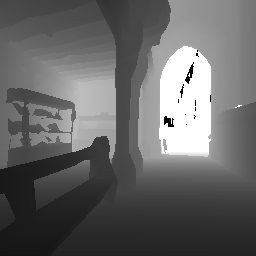
\includegraphics[width=\textwidth]{imagenes/cap5/normalized.png}
    \caption{Imagen normalizada.}
    \end{subfigure}
    \begin{subfigure}[b]{.475\textwidth}
    \centering
    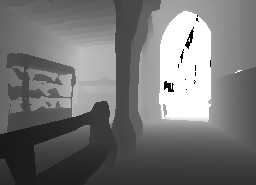
\includegraphics[width=\textwidth]{imagenes/cap5/trimmed.png}
    \caption{Imagen recortada.}
    \end{subfigure}
    
    \begin{subfigure}[b]{.475\textwidth}
    \centering
    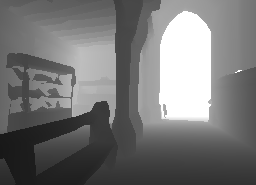
\includegraphics[width=\textwidth]{imagenes/cap5/filled.png}
    \caption{Imagen sin artefactos.}
    \end{subfigure}
    \begin{subfigure}[b]{.475\textwidth}
    \centering
    
\includegraphics[width=\textwidth]{imagenes/cap5/thresholded.png}
    \caption{Imagen con umbral aplicado.}
    \end{subfigure}

	\begin{subfigure}[b]{.475\textwidth}
    \centering
    
\includegraphics[width=\textwidth]{imagenes/cap5/cleaned.png}
    \caption{Imagen sin ruido.}
    \end{subfigure}
    \begin{subfigure}[b]{.475\textwidth}
    \centering
    
\includegraphics[width=\textwidth]{imagenes/cap5/dilated.png}
    \caption{Imagen dilatada.}
    \end{subfigure}

    \caption{Procesamiento realizado sobre la imagen de profundidad.}
    \label{fig:chap5-imageprocess}
\end{figure*}

\subsubsection{Identificación de los obstáculos y la distancia en la imagen}

Tras el preprocesamiento de la imagen, es necesario identificar los obstáculos en la imagen   y estimar la distancia a la que éstos se encuentran. Para eso, se han propuesto dos métodos:

\begin{itemize}
	\item \textbf{Método de contornos:} Este método se basa en la propuesta original de Carlos Sampedro \textit{et al.} \cite{Sampedro2018}. 
	
	La idea principal del método es identificar los contornos que tengan un área mínimo (experimentalmente determinado como $250$ pixeles) en la imagen preprocesada. A partir de estos contornos, se crean máscaras en la imagen original para extraer los obstáculos de nuevo en escala de grises. Finalmente, se obtiene la cercanía de esos obstáculos (a partir del pixel de valor mínimo), usando la siguiente estimación:
	\[distancia = \frac{(pixel\_min / 256) * distancia\_estimada}{umbral\_obstaculo}\]
Donde $pixel\_min$ es el pixel de menor valor en el obstáculo (en el rango ${0, 255}$), $distancia\_estimada$ es un valor heurístico que indica la distancia a la que se encontraría un obstáculo en el umbral (estimado como $2$ metros) y $umbral\_obstaculo$ es el umbral que se ha usado durante la umbralización ($0.15$).

Se puede ver el pseudocódigo del proceso en la Figura \ref{alg:contour}.

\begin{figure}[h]
\begin{algorithm}[H]
\SetAlgorithmName{Algoritmo}{algoritmo}{Lista de algoritmos}
\caption{Identificación de distancias con método de contornos}
\textbf{Variables:} Imagen preprocesada $imagen\_p$, imagen recortada $imagen\_r$, umbral usado durante preprocesamiento $umbral$, distancia estimada hasta el umbral en metros $dist$, área mínima de los contornos en píxeles $area\_min$.\\
\textbf{1.} Inicializa una lista para almacenar las distancias obtenidas, $distancias$.\\
\textbf{2.} Extrae los contornos de la imagen $imagen\_p$ a una lista $contornos$.\\
\textbf{3.} Para cada contorno $cont$ de area $area\_contorno$ en $contornos$, con $area\_contorno \geq area\_min$:\\
\Indp \textbf{3.1.} Aplica una máscara con la forma de $cont$ a $imagen\_r$, obteniendo el obstáculo $obs$ (el obstáculo tal y como está representando en la imágen $imagen\_r$, en escala de grises).\\
\textbf{3.2.} Obtén la distancia mínima en $obs$ (el valor mínimo), $dist\_obs$.\\
\textbf{3.3.} Convierte $dist\_obs$ de un valor entero en el rango $\{0, 255\}$ a una distancia en metros mediante una equivalencia usando $umbral$ y $dist$.\\
\textbf{3.4.} Si $dist\_obs \leq dist$, almacena $dist\_obs$ en $distancias$.\\
\Indm \textbf{4.} Devuelve $distancias$.
\end{algorithm}
\hrule
\caption{Pseudocódigo del método de contornos para identificar distancias a obstáculos.}
\label{alg:contour}
\end{figure}

\newpage 

	\item \textbf{Método de columnas:} Un método original, consistente en dividir la imagen  en columnas de misma anchura, siendo cada columna un posible obstáculo. 
	
	El método consiste en dividir la imagen preprocesada en $8$ (elegido experimentalmente) columnas de anchura idéntica. Tras esto, se cuenta el número de píxeles blancos (obstáculos) en cada columna, considerando las columnas que tengan una cantidad superior al área mínima ($250$ píxeles como se ha mencionado previamente) como obstáculos. Para estas columnas, se estima la distancia a partir de una columna equivalente de la imagen original, usando la fórmula descrita previamente:
	\[distancia = \frac{(pixel\_min / 256) * distancia\_estimada}{umbral\_obstaculo}\]
Donde $pixel\_min$ es el pixel de menor valor en el obstáculo (en el rango ${0, 255}$), $distancia\_estimada$ es un valor heurístico que indica la distancia a la que se encontraría un obstáculo en el umbral (estimado como $2$ metros) y $umbral\_obstaculo$ es el umbral que se ha usado durante la umbralización ($0.15$).

Se puede ver el pseudocódigo del proceso en la Figura \ref{alg:column}.

\begin{figure}[h]
\begin{algorithm}[H]
\SetAlgorithmName{Algoritmo}{algoritmo}{Lista de algoritmos}
\caption{Identificación de distancias con método de columnas}
\textbf{Variables:} Imagen preprocesada $imagen\_p$, imagen recortada $imagen\_r$, umbral usado durante preprocesamiento $umbral$, distancia estimada hasta el umbral en metros $dist$, área mínima de los contornos en píxeles $area\_min$.\\
\textbf{1.} Divide las imágenes $imagen\_p$ y $imagen\_r$ en columnas de anchuras iguales, $columnas\_p$ y $columnas\_r$.\\
\textbf{2.} Para cada columna $col$ con $pixeles$ pixeles blancos en $columnas\_p$ y $col\_r$ en $columnas\_r$, cumpliendo que $pixeles \geq area\_min$:\\
\Indp\textbf{2.1.} Obtén la distancia mínima en $col\_r$ (el valor mínimo), $dist\_obs$.\\
\textbf{2.2.} Convierte $dist\_obs$ de un valor entero en el rango $\{0, 255\}$ a una distancia en metros mediante una equivalencia usando $umbral$ y $dist$.\\
\textbf{2.3.} Si $dist\_obs \leq dist$, almacena $dist\_obs$ en $distancias$.\\
\Indm \textbf{3.} Devuelve $distancias$.
\end{algorithm}
\hrule
\caption{Pseudocódigo del método de columnas para identificar distancias a obstáculos.}
\label{alg:column}
\end{figure}

Este método se propone al considerar que el método anterior daría la misma importancia a un obstáculo grande (que ocupa gran parte de la pantalla) y a uno pequeño siempre y cuando estuviesen a la misma distancia. La idea es remediar ese problema, dando más peso a los obstáculos más grandes. Además, al evitar tener que usar algoritmos de búsqueda de contornos, se espera que la velocidad de ejecución sea mayor.

\end{itemize}

\subsubsection{Cálculo del potencial atractivo y repulsivo}

Tras el cálculo de las distancias a los obstáculos, se calcula el valor de los potenciales atractivos y repulsivos. Este cálculo es equivalente al propuesto por Carlos Sampedro \textit{et al.} \cite{Sampedro2018} originalmente.

El \textbf{potencial atractivo} es la fuerza con la que la meta atrae al agente. Cuanto más cerca esté el agente de la meta, mayor debe ser su influencia. Este potencial se obtiene con la siguiente fórmula:
\[U_{atr} = \alpha p_{goal}(t_r)\]
Donde $\alpha$ es una ganancia positiva usada para aumentar la influencia del potencial (estimada empíricamente como $100$) y $p_{goal}(t_r)$ es la distancia euclídea entre la posición actual del agente y la meta.

El \textbf{potencial repulsivo} es la suma de las fuerzas con las que los obstáculos repelen al agente. Cuantos más obstáculos perciba el agente y más cerca se encuentren, mayor debe ser su influencia. Este potencial se obtiene con la siguiente fórmula:
\[U_{rep} = \beta \sum_{i=1}^{N}(\frac{1}{k+l_i}-\frac{1}{k+l_{max}})\]
Donde $N$ es el número total de obstáculos detectados, $k$ es una constante usada para limitar la influencia de los obstáculos (con valor por defecto $0.04$), $l_i$ es la distancia al obstáculo $i$ en metros, $l_{max}$ es la distancia máxima a la que se detectan los obstáculos (con valor por defecto $2$ metros) y $\beta$ se obtiene con la siguiente fórmula:
\[
\beta = 
\begin{cases}
\delta,& \text{si } p_{goal}(t_r) > d_{infl}\\
\frac{\delta}{exp[4(d_{infl}-p_{goal})]},& \text{si } p_{goal}(t_r) \leq d_{infl}
\end{cases}
\]
Donde $\delta$ es una ganancia positiva usada para aumentar la influencia del potencial (estimada empíricamente como $15$) y $d_{infl}=0.75 l_{max}$ es una distancia a partir de la cual la influencia del potencial repulsivo se disminuye, para fomentar al agente a acercarse a la meta cuando se encuentra próximo a ésta.

Tras el cálculo de ambos potenciales, es posible calcular el \textbf{valor del estado actual}. Cuanto mayor es el valor del estado, mejor estado se considera que es. Este valor se comparará con el valor del estado previo para comprobar si ha mejorado o empeorado, y obtener una recompensa a partir de ello.

Este valor se calcula como:
\[valor_t=-U_{atr}-U_{rep}\]

\subsubsection{Cálculo de la recompensa final}
 
Tras haber calculado los potenciales y el valor del estado, es posible obtener la recompensa final a partir de las siguientes reglas:

\begin{itemize}

\item Si el episodio ha finalizado (ya sea por la acción correspondiente o por limite de acciones) y el agente no está en rango de la meta: \textbf{-100}.

La penalización por finalizar un episodio sin éxito es muy alta para evitar que el agente finalice el episodio antes de tiempo con la intención de evitar penalizaciones por sus acciones.

\item Si el episodio ha finalizado (ya sea por la acción correspondiente o por límite de acciones) y el agente está en rango de la meta: \textbf{+10}.

La recompensa por finalizar un episodio con éxito es menor, pero sigue siendo elevada para fomentar al agente a llegar a la meta y finalizar en ella.

\item En cualquier otro caso:

Si el episodio no ha finalizado tras la acción del agente, se procede a calcular la recompensa a partir de los valores del estado actual y el previo:
\[recompensa = (valor_t - valor_{t-1}) - 0.25, \text{acotado en el rango } [-100, +10]\]

Si el valor del estado alcanzado tras realizar la acción es mayor (la acción lleva a un estado mejor) la recompensa será positiva, mientras que si el valor es menor (la acción lleva a un estado peor) la recompensa será negativa. De esta forma, se fomenta que el agente intente mejorar su posición continuamente.

El término $-0.25$ es una penalización por paso, usada para evitar que el agente permanezca en bucles infinitos sin recompensa y acelerando su progreso.

\end{itemize} 

Una alternativa propuesta es incluir una regla adicional al cálculo de recompensas:
\begin{itemize}
	\item Si el agente ha colisionado con algún obstáculo tras la acción: \textbf{-100} y \textbf{finaliza el episodio}.
	
	Con esta regla adicional, se penaliza notablemente que el agente colisione con los obstáculos, fomentando que evite cualquier colisión con el entorno. Estas colisiones se comprueban usando la métrica \textit{COLLISIONS}.
\end{itemize}

\newpage

\section{Arquitectura del agente}

En esta sección se discuten las arquitecturas (redes neuronales) propuestas para el agente, su funcionamiento y su implementación. Se han propuesto dos arquitecturas, de las cuales se ha elegido una finalmente:

\begin{itemize}
		\item Una primera aproximación basada en \textbf{redes neuronales convolucionales}.
		\item Una segunda aproximación basada en un \textbf{enfoque mixto}, con redes convolucionales y redes neuronales densas tradicionales.
\end{itemize}

\subsection{Propuesta 1: Red convolucional (CNN)}

La primera aproximación está basada en el uso de \textbf{redes convolucionales \textit{(CNNs)}} para el procesamiento de la imagen, extrayendo las características profundas relevantes para trabajar posteriormente con ellas. 

Ahora bien, los valores numéricos (parte del estado a procesar) no pueden ser usados directamente por las capas de convolución. Para solventar esto, los dos valores numéricos (distancia y ángulo) son concatenados directamente a la salida aplanada de las convoluciones, para ser procesados posteriormente por las capas densas de neuronas.

La arquitectura de la red neuronal se ha basado en la arquitectura original de \textit{AlexNet} \cite{Krizhevsky2012ImageNetCW}, adaptada de forma \textit{ad-hoc} para las necesidades del trabajo y las limitaciones existentes de memoria y tiempo.

La red se puede dividir en varias secciones consecutivas:
\begin{enumerate}
	\item \textbf{Entrada:} La entrada se obtiene de una muestra del \textit{Experience Replay}. Cada elemento de esta muestra es un estado, correspondiendose con la definición dada previamente de estado:
	\begin{itemize}
		\item Una imagen de profundidad (escala de grises), en forma de una matriz bidimensional de tamaño $256x256$ con una única capa.
		\item Dos valores escalares: la distancia y el ángulo hasta la meta.
	\end{itemize}
	
	\item \textbf{Convolución:} El primer paso de la red es procesar la imagen a través de varios procesos de convolución, con el fin de obtener las características profundas de ésta. Para esto, se tienen \textbf{tres} procesos de convolución consecutivos, cada uno de ellos formado por, en orden:
		\begin{itemize}
			\item Capa convolucional bidimensional de 16 filtros. El tamaño del \textit{kernel} es de $5x5$, $3x3$ y $3x3$ en cada proceso respectivamente.
			\item Función de activación ReLU.
			\item Capa de \textit{pooling} por función de máximo. El tamaño del \textit{pooling} es de $3x3$, $3x3$ y $2x2$ en cada proceso respectivamente.
		\end{itemize}
		
	A pesar de ser típico en redes convolucionales, no se ha incluido ninguna capa de \textit{batch normalization} durante el proceso de convolución. Ésto se debe a que el proceso de normalización introduce ruido que puede alterar el proceso de aprendizaje por refuerzo \cite{Salimans2016}.
	
	\item \textbf{Aplanado (\textit{Flatten}):} Tras la convolución de la imagen, el resultado del proceso (una matriz tridimensional profunda con las características de la imagen) es aplanado a un conjunto unidimensional de neuronas. Esto permite a las capas posteriores trabajar con la información obtenida. Esta capa no cuenta con ninguna función de activación.
	
	En este paso además se concatenan los dos valores escalares de la entrada (distancia y ángulo a la meta). Estos valores no han sido incluidos previamente al no poder ser procesados por las capas convolucionales. Al añadirlos ahora, las capas posteriores podrán trabajar con la información.
	
	\item \textbf{Capas densas:} Tras el aplanamiento y concatenación de la información en el paso previo, se incluyen \textbf{dos} capas densas (capas de neuronas totalmente conectadas) para extraer relaciones entre la información obtenida.
	
	Estas capas densas cuentan con $256$ neuronas cada una, utilizando \textit{ReLU} como función de activación.
	
	\item \textbf{Salida:} Finalmente, la capa de salida es una capa densa de cuatro neuronas, donde cada neurona se corresponde con el valor Q de una de las cuatro acciones disponibles para el agente. Estas neuronas cuentan con función de activación lineal.
\end{enumerate}

Se puede observar un esquema de la arquitectura en la Figura \ref{fig:chap5-arc1}.

\begin{figure}
    \centering
    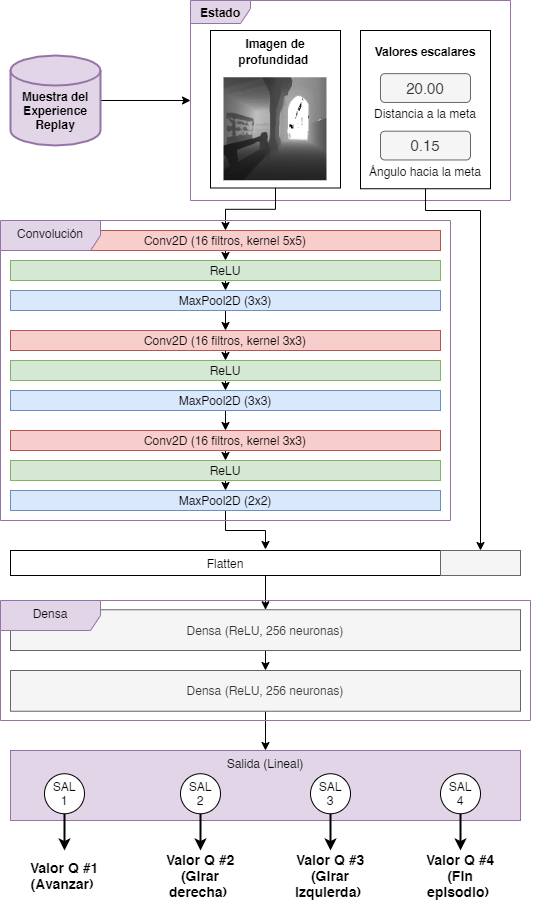
\includegraphics[height=0.95\textheight]{imagenes/cap5/arquitectura1.png}
    \caption{Arquitectura de la red neuronal - Propuesta 1 (CNN).}
    \label{fig:chap5-arc1}
\end{figure}	

La red neuronal ha sido implementada utilizando las librerías \textit{TensorFlow} y \textit{Keras}. Para las funciones usadas por la red para su entrenamiento, se ha optado por utilizar algunos algoritmos tradicionalmente usados en problemas de aprendizaje profundo, siendo éstos:
\begin{itemize}
	\item \textbf{Función de inicialización de pesos:} Glorot y Bengio \cite{Glorot2010UnderstandingTD}.
	\item \textbf{Función de optimización:} Adam \cite{adam2014}.
	\item \textbf{Función de error:} Error cuadrático medio. Esta función de error es usada tradicionalmente en problemas de aprendizaje por refuerzo profundo.
\end{itemize}

Tras realizar pruebas iniciales (entrenamientos cortos) con la arquitectura propuesta, se observaron una serie de problemas con ésta:

\begin{itemize}
	\item \textbf{Ineficiencia en memoria:} Debido al tamaño de la red y a problemas con la librería utilizada, el uso de memoria (tanto memoria \textit{RAM} del ordenador como de la \textit{GPU}) era excesivo. Además, este uso crecía tras cada episodio hasta llegar a un punto en el que se detenía el entrenamiento por falta de memoria.
	
	Esto provocaba que no fuese posible realizar entrenamientos largos, y que los entrenamientos realizados fuesen notablemente más lentos de lo esperado.
	\item \textbf{Malos resultados:} Durante el proceso de entrenamiento se observó que los resultados obtenidos por la red eran peores de lo que se podría esperar, sin mostrar signos de aprendizaje. Esto se puede deber al uso de los valores escalares, al ser menos relevantes (2 neuronas) frente a la información obtenida de la imagen (miles de neuronas).
\end{itemize}

Por estos problemas, se ha optado por \textbf{descartar} esta arquitectura en favor de la segunda propuesta, descrita a continuación. La implementación de esta propuesta se conserva en los ficheros \textit{models/DEPRECATED{\_}reactive{\_}navigation{\_}keras.py} y \textit{trainers/DEPRECATED{\_}reactive{\_}navigation{\_}trainer{\_}keras.py}, por motivos de documentación

\subsection{Propuesta 2: Red mixta (CNN + MLP)}

La segunda aproximación está basada en el uso de \textbf{redes híbridas} (es decir, redes formadas por varias redes neuronales más pequeñas).

Una red convolucional no está preparada para trabajar con valores escalares numéricos. Ahora bien, un perceptrón multicapa (\textit{MLP}) estándar no puede procesar imágenes con el mismo rendimiento que una red convolucional. Por tanto, una de las mejores opciones para trabajar con entradas mixtas de imágenes y valores escalares es procesar cada tipo de entrada en una red neuronal separada específica (las imágenes en redes convolucionales y los valores escalares en redes densas), obteniendo resultados que serán juntados y procesados posteriormente en una red neuronal final.

La arquitectura de esta propuesta está inspirada por las arquitecturas propuestas para resolver otros problemas con entrada mixta de imágenes y valores numéricos, como el trabajo de Md Manjurul Ahsan \textit{et al.}  para distinguir casos de COVID-19 \cite{sym12091526} o el trabajo de Yanyu Zhang aplicando redes mixtas al aprendizaje por refuerzo profundo \cite{DBLP:journals/corr/abs-2010-00717}. Se ha desarrollado la arquitectura de forma \textit{ad-hoc} para las necesidades del proyecto.

La propuesta consta con dos redes neuronales (una red convolucional y un perceptrón multicapa) que procesan sus entradas de forma paralela. Tras esto, las salidas de ambas redes se pasan a una red final que obtiene el resultado. La arquitectura de las tres redes son las siguientes:

\begin{itemize}

\item \textbf{Red convolucional (CNN):} Esta red se encarga del procesamiento de la imagen de profundidad de la entrada, extrayendo las características profundas de ésta para ser aprovechadas posteriormente. Consta de las siguientes capas:
\begin{enumerate}
	\item \textbf{Entrada:} La entrada es una imagen de profundidad (escala de grises) en forma de matriz bidimensional de tamaño $256x256$, con una única capa. Esta imagen se obtiene de los estados muestreados del \textit{Experience Replay}.
	\item \textbf{Convolución:} El primer paso de la red es procesar la imagen para extraer las características principales, reduciendo su tamaño. Para esto se usan \textbf{tres} procesos de convolución consecutivos, cada uno de ellos formado por, en orden:
	\begin{itemize}
		\item Capa convolucional bidimensional. El número de filtros depende del proceso de convolución, siendo éste de $16$, $32$ y $16$ filtros respectivamente. El tamaño del $kernel$ también varía dependiendo del proceso, siendo éste de $5x5$, $3x3$ y $3x3$ en cada proceso respectivamente.
		\item Función de activación ReLU.
		\item Capa de \textit{pooling} con función de máximo. El tamaño de \textit{pooling} es de $3x3$, $3x3$ y $2x2$ respectivamente dependiendo del proceso de convolución.
	\end{itemize}
	\item \textbf{Aplanado (\textit{Flatten}):} Tras la convolución de la imagen, es necesario aplanar el resultado (la matriz tridimensional con las características identificadas) a un conjunto unidimensional de neuronas. Este aplanamiento permite a las capas densas posteriores trabajar de forma correcta con la información. Esta capa no cuenta con ninguna función de activación.
	\item \textbf{Capa densa:} En este caso, tras el aplanado hay una única capa densa (capa de neuronas totalmente conectadas) de \textbf{64} neuronas usando \textbf{ReLU} como función de activación. Con esta capa se busca identificar relaciones existentes entre las características encontradas previamente con la convolución.
	\item \textbf{Salida:} La capa de salida es una única capa densa con tres neuronas, con función de activación lineal. Se ha optado por utilizar una función de activación lineal para no modificar el valor de salida alcanzado de ninguna manera, buscando evitar sesgos.
	
	Estas neuronas posteriormente servirán como entrada para otra red neuronal.
\end{enumerate}

\item \textbf{Red neuronal profunda / Perceptrón multicapa (MLP):} Esta red se encarga del procesamiento de los valores numéricos de la entrada, preparándolos para su uso posterior. Consta de las siguientes capas:

\begin{enumerate}
\item \textbf{Entrada:} La entrada son dos valores numéricos (la distancia y el ángulo hacia la meta), obtenidos de los estados muestreados del \textit{Experience Replay}.
\item \textbf{Capas ocultas:} Tras la entrada, la red cuenta con \textbf{dos} capas densas (neuronas totalmente conectadas) de \textbf{diez} neuronas cada una, con función de activación ReLU. Estas capas de neuronas se encargan de procesar las entradas numéricas.

El número de neuronas se ha obtenido a partir del número de entradas y salidas, siendo $2(entrada + salida) = 10$.
\item \textbf{Salida:} La capa de salida es una única capa densa con tres neuronas, con función de activación lineal. De nuevo, se utiliza una función de activación lineal para que el valor de las neuronas de salida no se vea modificado de ninguna forma.

Estas neuronas serán usadas posteriormente como entrada para otra red neuronal.
\end{enumerate}

\item \textbf{Red mixta (CNN + MLP):} Esta red toma las salidas de las dos redes anteriores, juntándolas y procesándolas para obtener las salidas finales de la red neuronal. La arquitectura de esta red es una red neuronal estándar, con las siguientes capas:
\begin{enumerate}
\item \textbf{Concatenación / Entrada:} La entrada de la red es una concatenación de las salidas de las dos redes neuronales anteriores: \textbf{3} neuronas de la imagen procesada y \textbf{3} neuronas de los valores numéricos procesados, para un total de \textbf{6} neuronas. Esta capa no tiene ninguna función de activación.

Se ha decidido que ambas redes neuronales tengan el mismo número de neuronas en la salida para que ambas partes del estado (imagen y valores numéricos) tuviesen la misma relevancia a la hora de obtener una salida. Además, se ha elegido usar \textbf{tres} neuronas en cada salida por tener un número pequeño de neuronas, pero suficientemente grande para que haya una expresión rica de características.
\item \textbf{Capas ocultas:} Tras la entrada, la red cuenta con \textbf{dos} capas densas de \textbf{32} neuronas, con funciones de activación ReLU.

Se ha optado por utilizar dos capas con un número moderado de neuronas frente a una capa con una gran cantidad de neuronas por ofrecer mejor rendimiento, dando la posibilidad con más capas de encontrar más relaciones entre datos.
\item \textbf{Salida:} La capa de salida es una capa densa de cuatro neuronas, donde cada neurona se corresponde con el valor Q de una de las cuatro acciones disponibles para el agente. Esta capa utiliza una función de activación lineal.
\end{enumerate}

\end{itemize}

Se puede observar un esquema de la arquitectura en la Figura \ref{fig:chap5-arc2}.

\begin{figure}
    \centering
    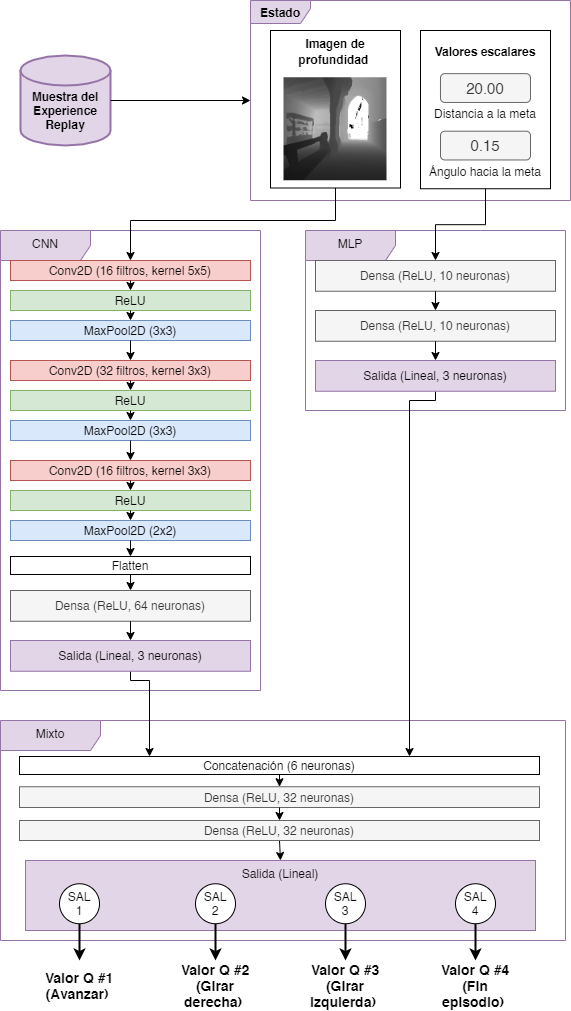
\includegraphics[height=0.95\textheight]{imagenes/cap5/arquitectura2.png}
    \caption{Arquitectura de la red neuronal - Propuesta 2 (Mixta).}
    \label{fig:chap5-arc2}
\end{figure}	

A diferencia de la propuesta anterior, la red neuronal ha sido implementada utilizando la librería \textit{PyTorch}, estando disponible la implementación en el fichero \textit{models/reactive{\_}navigation.py}. Para las funciones usadas por la red durante su entrenamiento, se han usado algoritmos más novedosos que los de la propuesta anterior, siendo estos:

\begin{itemize}
	\item \textbf{Función de inicialización de pesos:} Kaiming \cite{DBLP:journals/corr/HeZR015}.
	\item \textbf{Función de optimización:} Adam \cite{adam2014}.
	\item \textbf{Función de error:} Error de Huber \cite{10.1214/aoms/1177703732}. 
	
	Esta función es una variante del error cuadrático medio propuesta por Huber en 1964, siendo más resistente a los valores aislados. Concretamente, la función es cuadrática para valores residuales pequeños, mientras que se vuelve lineal para valores elevados.
\end{itemize}

Esta propuesta ha sido elegida como la arquitectura definitiva usada por el agente, al ofrecer mejores resultados en un tiempo de entrenamiento menor, sin ningún error ni problema durante la ejecución.

\section{Actuación del agente}

El proceso de actuación del agente está basado en el proceso de actuación estándar de un agente de \textit{Deep Q-Learning} siguiendo el paradigma de exploración / explotación, pudiendo ser observado en la Figura \ref{alg:act}.

\begin{figure}[h]
\begin{algorithm}[H]
\SetAlgorithmName{Algoritmo}{algoritmo}{Lista de algoritmos}
\caption{Actuación del agente}
\textbf{Entradas:} Estado $s$, formado por una imagen de profundidad $depth$ y dos valores numéricos, la distancia a la meta $dist$ y  el ángulo hacia la meta $angle$.\\
\textbf{Variables internas del agente:} Probabilidad de acción aleatoria $\epsilon$, lista de acciones posibles $action\_list$.
 el agente conserva una variable $\epsilon$ para el ratio de exploración / explotación.\\
\textbf{1.} Genera un valor aleatorio $rand$ en el rango $[0.0, 1.0]$.\\
\textbf{2.} Si $rand < \epsilon$:\\
\Indp \textbf{2.1} Exploración. Se elige una acción $action$ de $action\_list$ aleatoriamente, siguiendo una distribución uniforme.\\
\Indm \textbf{3.} En otro caso ($rand \geq \epsilon$):\\
\Indp \textbf{3.1.} Explotación. Procesa el estado $s$ a través de la red neuronal, obteniendo la lista de valores Q para cada par estado-acción $q\_values$.\\
\textbf{3.2.} Elige la acción $action$ de $action\_list$ que tenga el máximo valor en $q\_values$.\\
\Indm \textbf{4.} Devuelve $action$.
\end{algorithm}
\hrule
\caption{Proceso de actuación del agente.}
\label{alg:act}
\end{figure}

Como ya se ha mencionado, la actuación del agente sigue el paradigma de exploración-explotación, usando $\epsilon$ como la variable que regula el proceso. $\epsilon$ se actualiza durante el entrenamiento tras cada episodio siguiendo la siguiente fórmula:
\[\epsilon= max\left( \frac{(\epsilon_{init} - \epsilon_{min}) * porcentaje}{\epsilon_{min\_porcentaje}} - \epsilon_{init}, \epsilon_{min} \right)\]
Donde $\epsilon_{init}$ es el valor inicial de $\epsilon$ (por defecto $1.0$), $\epsilon_{min}$ es el valor mínimo alcanzado por $\epsilon$ (por defecto $0.05$), $\epsilon_{min\_porcentaje}$ es el porcentaje de episodios tras el cual el valor de $\epsilon$ alcanzará $\epsilon_{min}$ (por defecto $0.8$, el $80\%$ de los episodios) y $porcentaje$ es el porcentaje actual de episodios completados.

En esencia, el valor de $\epsilon$ decrece linealmente desde su valor inicial, $\epsilon_{init}$, hasta su valor final, $\epsilon_{min}$, conforme el agente completa episodios. El valor final será alcanzado tras completar el $\epsilon_{min\_porcentaje}\%$ de los episodios (por ejemplo, para un entrenamiento de 10.000 episodios $\epsilon_{min}$ se alcanzaría a los 8000 episodios). El valor de $\epsilon$ no puede bajar de $\epsilon_{min}$ en ningún momento.

El objetivo es que en los primeros episodios el agente explore una gran cantidad de estados (\textbf{exploración}) mientras no tiene suficiente conocimiento como para tener una política de acciones de calidad. Conforme el agente completa episodios y adquiere conocimiento, se busca que éste empiece a aprovechar las experiencias previas en los episodios finales (\textbf{explotación}), efectuando menos acciones aleatorias y más acciones acordes a la política aprendida.

Cuando el agente es usado fuera de un entorno de entrenamiento (como puede ser durante su evaluación), el valor de $\epsilon$ se queda fijado como $\epsilon=0$, para explotar totalmente la política sin ninguna acción aleatoria.

\section{Entrenamiento del agente}

En esta sección se describe el proceso seguido por el agente para realizar su entrenamiento. El agente ha sido entrenado utilizando el algoritmo de \textit{Deep Q-Learning}, siendo el pseudocódigo del algoritmo el expuesto en la Figura \ref{alg:chap5-dql}.

\begin{figure}[h]
\begin{algorithm}[H]
\SetAlgorithmName{Algoritmo}{algoritmo}{Lista de algoritmos}
\caption{Entrenamiento del agente}
\textbf{Variables iniciales:} Dos agentes, un agente conteniendo la red Q, $agente\_q$, y un agente conteniendo la red objetivo, $agente\_obj$. \textit{Experience Replay} $exp\_replay$ donde se almacenan las experiencias del agente. Número total de episodios a realizar durante el entrenamiento, $ep\_total$. $\epsilon$, probabilidad de realizar una acción aleatoria.\\
\textbf{1.} Inicializa un contador, $cont\_ep=0$, para almacenar el numero de episodios realizados hasta el momento.\\
\textbf{2.} Mientras $cont\_ep < ep\_total$:\\
\Indp \textbf{2.1} Inicializa el episodio $episodio$, obteniendo el estado inicial $estado$.\\
\textbf{2.2} Mientras $episodio$ no haya finalizado:\\
\Indp \textbf{2.2.1.} $agente\_q$ elige la acción $accion$ a realizar para $estado$ dependiendo de $\epsilon$, usando el método descrito previamente.\\
\textbf{2.2.2.} Se aplica $accion$ a $estado$, obteniendo una recompensa $recompensa$, un nuevo estado $n\_estado$ y un indicador de si $n\_estado$ es final, $final$.\\
\textbf{2.2.3.} Se almacena $estado$, $accion$, $recompensa$, $n\_estado$ y $final$ en $exp\_replay$.\\
\textbf{2.2.4.} Se toma una muestra $batch$ de $exp\_replay$, y se entrena al agente $agente\_q$ a partir de $batch$, usando los resultados de $agente\_q$ y $agente\_obj$.\\
\textbf{2.2.5.} $estado=n\_estado$.\\
\Indm \textbf{2.3.} Actualiza $agente\_obj$ con los pesos de $agente\_q$.\\
\textbf{2.4.} Actualiza $\epsilon$.\\
\textbf{2.5.} $cont\_ep++$.\\
\textbf{2.6.} Documenta el proceso de entrenamiento.\\
\Indm \textbf{3.} Devuelve los pesos de $agente\_q$ como agente entrenado.
\end{algorithm}
\hrule
\caption{Proceso de entrenamiento del agente.}
\label{alg:chap5-dql}
\end{figure}

Se ha optado por utilizar \textit{Deep Q-Learning} frente a otras técnicas de aprendizaje por refuerzo profundo como \textit{PPO} principalmente por familiaridad con la técnica. Además, \textit{Deep Q-Learning} sigue ofreciendo buenos resultados en problemas de aprendizaje por refuerzo profundo, especialmente si se aplican mejoras como \textit{Prioritized Experience Replay}.

Se han planteado dos variantes para el entrenamiento, dependiendo de la técnica utilizada:
\begin{itemize}
	\item Entrenamiento usando \textit{Deep Q-Learning} estándar.
	\item Entrenamiento usando \textit{Deep Q-Learning} con \textit{Prioritized Experience Replay}.
\end{itemize}

A continuación, se describen los elementos principales del entrenamiento.

\subsection{\textit{Replay Memory} y memorización de la experiencia}

El \textit{Replay Memory} del agente se encarga de almacenar las experiencias previas del agente, para su muestreo posterior durante el entrenamiento. Estas experiencias son almacenadas con la forma $<s, a, r, s', f>$, siendo cada elemento:

\begin{itemize}
\item $s$: Estado inicial de la experiencia.
\item $a$: Acción aplicada sobre el estado $s$.
\item $r$: Recompensa obtenida tras aplicar la acción $a$ al estado $s$.
\item $s'$: Estado nuevo, alcanzado tras aplicar la acción $a$ al estado $s$.
\item $f$: Valor booleano que indica si $s'$ es un estado final (ha provocado el final del episodio) o no.
\end{itemize}

Internamente, el \textit{Replay Memory} es una cola FIFO estándar de tamaño $M$ (por defecto, $20000$ posiciones) donde se introducen las experiencias. Cuando la cola se llena, la introducción de una nueva experiencia provocará que la experiencia más antigua sea eliminada. De esta forma, se evita que el conocimiento del agente se estanque al ir renovando las experiencias conforme se van experimentando nuevas experiencias.

Tras cada actuación del agente, se introduce la experiencia (los valores descritos anteriormente) en la memoria y se realiza un proceso de aprendizaje como se verá posteriormente.

La variante usando \textit{Prioritized Experience Replay} presenta las siguientes diferencias:
\begin{itemize}
\item El \textit{Replay Memory} pasa de almacenar directamente la experiencia $<s, a, r, s', f>$ a una tupla $(experiencia, error)$. En esta tupla, $experiencia$ sigue teniendo la estructura $<s, a, r, s', f>$, pero $error$ simboliza el error que presenta la experiencia (siendo éste la diferencia entre los valores Q que se espera que devuelva la red para $s$ y los valores Q realmente obtenidos).
\item Cuando se inserta una experiencia en el \textit{Replay Memory}, se inserta inicialmente como $(experiencia, \infty)$ (es decir, un valor de error infinito). Esto se debe a que inicialmente no se conoce el error, por lo que se busca el error más alto posible para fomentar que el agente aprenda la experiencia.
\end{itemize}

\subsection{Aprendizaje a partir de las experiencias}

Tras la memorización de una experiencia, se realiza aprendizaje a partir de una muestra tomada del \textit{Experience Replay}, viéndose el proceso general en la Figura \ref{alg:chap5-apst}.

\begin{figure}
\begin{algorithm}[H]
\SetAlgorithmName{Algoritmo}{algoritmo}{Lista de algoritmos}
\caption{Aprendizaje a partir de la experiencia (estándar)}
\textbf{Variables iniciales:} \textit{Experience Replay} $exp\_replay$. Dos agentes, el agente con la red neuronal Q $agente\_q$ y el agente con la red neuronal objetivo $agente\_obj$. $\gamma$, el peso dado a las nuevas experiencias en \textit{Deep Q-Learning}.\\
\textbf{1.} Obtén una muestra $muestra$ de $exp\_replay$, de tamaño $M$. Si $tamaño(exp\_replay) < M$ \textbf{finaliza el proceso sin aprender.}\\
\textbf{2.} Obtén los valores Q $Q\_s$ para los estados actuales contenidos en $M$ usando al agente Q $agente\_q$.\\
\textbf{3.} Obtén los valores Q $Q\_s'$ para los estados alcanzados contenidos en $M$ usando al agente objetivo $agente\_obj$.\\
\textbf{4.} Para cada experiencia $exp$ de la muestra $M$, donde $exp\_a$ es la acción tomada en $exp$, $exp\_r$ es la recompensa obtenida en $exp$, $exp\_f$ es la indicación de si $exp$ fue final y $exp\_q$ y $exp\_q'$ son los valores Q para el estado actual y alcanzado de $exp$ (calculados previamente en $Q\_s$ y $Q\_s'$ respectivamente):\\
\Indp \textbf{4.1.} Actualiza el valor Q asociado a la acción $exp\_a$ en $exp\_s$ siguiendo la siguiente fórmula:
\[
exp\_q(exp\_a)=
\begin{cases}
	exp\_r,& \text{si } exp\_f \text{ (si la experiencia es final)}\\
	exp\_r + \gamma * max(exp\_q'),& \text{en cualquier otro caso}\\
\end{cases}
\]\\
\Indm \textbf{5.} Actualiza las predicciones de $agente\_q$ para los estados actuales de $M$ usando las nuevas predicciones $exp\_q$ (usando retropropagación).\\
\end{algorithm}
\hrule
\caption{Proceso de aprendizaje a partir de las experiencias (estándar).}
\label{alg:chap5-apst}
\end{figure}

Hay algunos detalles importantes que remarcar sobre el proceso:
\begin{itemize}
	\item Por defecto, el tamaño de la muestra es de $64 experiencias$. Se ha optado por no entrenar al agente hasta que el \textit{Replay Memory} contenga al menos 64 experiencias, como en la propuesta original de \textit{Deep Q Learning}, para evitar problemas con la subdivisión de las muestras (como se verá a continuación).
	\item El aprendizaje se realiza en \textit{batch} (en paralelo). Esto significa que todas las muestras son pasadas a través de la red neuronal de forma simultanea, aprovechando el paralelismo ofrecido por las GPUs y mejorando el rendimiento.
	\item Para mejorar el uso en memoria, cada muestra se divide en submuestras de menor tamaño (por defecto, muestras de $64$ experiencias se dividen en submuestras de $32$ experiencias), que son pasadas consecutivamente por la red neuronal.
	
	Esto se ha hecho para suplir los problemas de memoria que surgieron durante el entrenamiento (al no haber suficiente memoria para procesar todos los valores a través de la red neuronal al mismo tiempo), haciendo más eficiente el uso de memoria a costa del tiempo de entrenamiento. Aun así, el rendimiento es notablemente superior al de un entrenamiento no paralelo.
\end{itemize}

La variante usando \textit{Prioritized Experience Replay} presenta las siguientes diferencias respecto a la Figura \ref{alg:chap5-apst}:
\begin{itemize}
\item El muestreo de experiencias no sigue una distribución uniforme, sino que sigue la siguiente distribución, siendo la probabilidad de elegir una experiencia $i$:
\[P(i)=\frac{p_i^{\alpha}}{\sum_k p_k^{\alpha}}\]
Donde $p_i$ es la prioridad de la experiencia $i$ (siendo $p_i=\frac{1}{rango(i)}$, donde $rango(i)$ es la posición de la experiencia $i$ en el \textit{Replay Memory} si éste se ordena de mayor a menor error) y $\alpha$ es una constante que indica el el grado de priorización (por defecto $0.5$).

Esto significa que las experiencias con mayor error tienen más probabilidad de ser muestreadas.
\item Los valores Q actualizados son normalizados con un peso $w_i$, siendo el peso de la experiencia $i$:
\[w_i=\left(\frac{1}{N} \frac{1}{P(i)}\right)^{\beta}\]
Donde $N$ es el número total de experiencias en el \textit{Replay Memory} y $\beta$ es un factor para ajustar la influencia del peso (por defecto $0.5$).

Por tanto, la actualización de valores Q en el punto \textbf{4.1} pasa a ser:
\[
exp\_q(exp\_a)=
\begin{cases}
	exp\_r * w_i,& \text{si } exp\_f \text{ (si la experiencia es final)}\\
	(exp\_r + \gamma * max(exp\_q')) * w_i,& \text{en cualquier otro caso}\\
\end{cases}
\]
\item Tras la actualización de los pesos de la red neuronal Q, los errores de las experiencias muestreadas del \textit{Replay Memory} son actualizados. Estos errores son calculados usando el error cuadrático medio, siendo la fórmula:
\[error=(q\_esperado - q\_obtenido)^2\]
\end{itemize}

\subsection{Documentación del entrenamiento}

Al final de cada episodio, el agente documenta el progreso durante el entrenamiento, imprimiendo en un fichero las siguientes métricas:
\begin{itemize}
	\item ID del episodio.
	\item Duración del episodio (en segundos).
	\item Número de acciones realizadas durante el episodio.
	\item Distancia inicial y final hasta la meta.
	\item Distancia recorrida hasta la meta ($dist\_inicial - dist\_final$). Este valor puede ser negativo si la posición final del agente es más lejana que la inicial.
	\item Exitoso (\textbf{Verdadero} si el agente ha alcanzado la meta, \textbf{Falso} en cualquier otro caso).
	\item Recompensa media obtenida.
\end{itemize}

A partir de estas métricas se realizará un análisis del rendimiento del agente durante el entrenamiento en el Capítulo 6.

Además, el agente almacena registros de su progreso durante el entrenamiento (\textit{checkpoints}), almacenando un total de \textbf{100} \textit{checkpoints} a lo largo de todo el entrenamiento (aproximadamente uno cada 150 episodios). Estos \textit{checkpoints} (ficheros de formato \textit{.pt}) contienen la siguiente información:
\begin{itemize}
	\item Los pesos de la red neuronal objetivo.
	\item El fichero de configuración que se estaba utilizando durante el entrenamiento.
\end{itemize}

A partir de estos \textit{checkpoints} es posible reanudar el entrenamiento en cualquier momento, y usarlos como los pesos finales para el agente entrenado.